% !TeX spellcheck = en_US
\documentclass[french]{yLectureNote}

\title{Électromagnétisme 3}
\subtitle{Physique}
\author{Paulhenry Saux}
\date{\today}
\yLanguage{Français}
%jesse.groenen@cemes.fr
\professor{M.Brut}
\usepackage{graphicx}%-pour mettre des images
\usepackage[utf8]{inputenc}%encodage
\usepackage{geometry}%pour modifier les tailles et mettre a4paper
%\usepackage{awesomebox}%pour les boites d'exercices, de pbq et de croquis d\'esactiv\'e pour les TP de PC
\usepackage{tikz}%pour deiffner + d\'ependance de chemfig
% \usepackage{tabularx}%pour dimensionner automatiquement les tableaux avec variable X
\usepackage{awesomebox}%Pour les boites info, danger et autres
\usepackage{menukeys}%Pour deiffner les touches de Calculatrice
\usepackage{fancyhdr}%pour les en-t\^ete personnalis\'ees
\usepackage{blindtext}%pour les liens
\usepackage{hyperref}%pour les liens (\`a mettre en dernier)
\usepackage{caption}%pour la francisation de la l\'egende table vers Tableau
\usepackage{pifont}
\usepackage{array}%pour les tableaux
\usepackage{lipsum}
\usepackage{yFlatTable}
\usepackage{multicol}
\usepackage{tabularx}
\usepackage{booktabs}
\usepackage{esint}
\newcommand{\Lim}[1]{\lim\limits_{\substack{1}}\:}
\renewcommand{\vec}{\overrightarrow}
\newcommand{\N}[0]{\mathbb{N}}
\newcommand{\dd}{\mathrm{d}}
\newcommand{\norm}[1]{||\vec{1}||}
\newcommand{\fo}{\psi(\vec{r},t)}
\newcommand{\HH}{\hat{H}}
\newcommand{\hb}{\hbar}
\newcommand{\lap}{\nabla^2}
\newcommand{\lapcc}{\frac{\partial^2 }{\partial x^2}+\frac{\partial^2 }{\partial y^2}+\frac{\partial^2 }{\partial z^2}}
\newcommand{\E}{\vec{E}(M)}
\newcommand{\B}{\vec{B}(M)}
\newcommand{\V}{V(M)}
\newcommand{\er}{\vec{e_{\rho}}}
\newcommand{\ez}{\vec{e_{z}}}
\newcommand{\ep}{\vec{e_{\varphi}}}
\newcommand{\pip}{\pi^+}
\newcommand{\pim}{\pi^-}
\newcommand{\mv}{\mathcal{V}}
\DeclareMathOperator{\Div}{Div}
\newcommand{\rot}{\vec{\mathrm{rot}}}
\newcommand{\grad}{\vec{\mathrm{grad}}}
\newcommand{\vds}{\vec{\dd S}}
\newcommand{\Ea}{\vec{E_{aux}}}
%\setcounter{chapter}{3}
\begin{document}

\chapter{Ferromagnétisme}


On a n atomes par unité de volume. Chaque atome porte un moment magnétique quantifié dont la projection est $\pm \mu_B$ qui est le magnéton de Bohr.

Dans le cadre de la théorie de Brillouin, on négligle les intéractions entre moments magnétiques sont négligées.

Les moments magnétiques sont donc indépendants. L'aimantation volumique vaut $M_{\infty}\tanh(X)$ avec $X=\frac{\mu_B B_a}{k_B T}$

$M_{\infty}$ est le moment à saturation volumique. On a $M_{\infty}=n\mu_b$.

On utilise le modèle du champ moyen de Weiss. L'intéraction d'échange entre moment magnétique est modélisée à l'aide d'un champ magnétique supplémentaire qui s'appelle $\vec{B_e} =\mu_0\lambda\vec{M}$, ce qui correspond au champ moyen de Weiss.

On traite chaque moment comme s'il était indépendant en le soumettant à un champ magnétique $\vec{B} = \vec{B_a}+\vec{B_e}$. On applique ensuite la théorie de Brillouin. 

Plus l'aimantation est importante, plus la contribution des autres moments est forte. Cest autres moments sont indépendants donc on peut utiliser la théorie de Briullouin.

Par analyse dimensionnelle, on se rend compte que $\lambda$ est sans dimension.

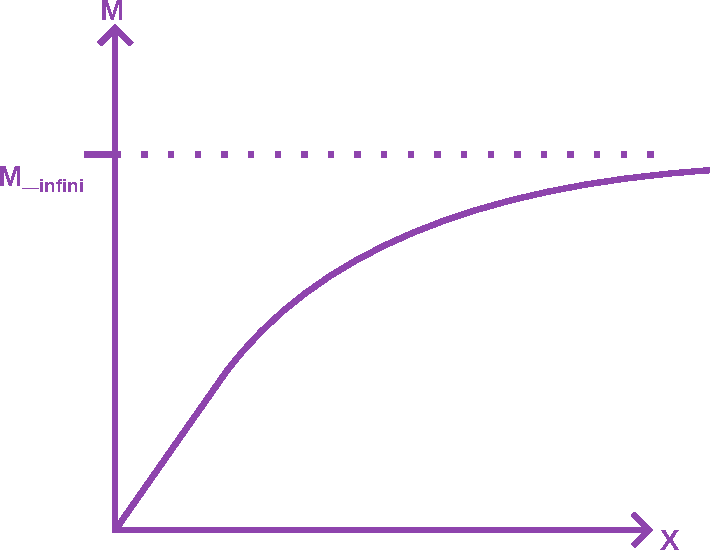
\includegraphics[scale=0.5]{m_ninfi.pdf}
\subsection{Comportement paramagnétique}
On se place en haute température, donc on peut faire l'approximation que $\th(X)\simeq X$. On peut donc écrire
$$M = \frac{n\mu_B^2}{k_BT}(B_a+\mu_0\lambda M)$$
Il faut donc extraire M puis introduire la suceptibilité. 
On obtient 
$$M(k_bT-n\lambda\mu_B^2\mu_0) =n\mu_B^2B_a$$

On obtient finalement
$$M = \frac{n\mu_B^2}{k_B(T-\frac{\mu_0\lambda n\mu_b^2}{k_B})} = \frac{n\mu_B^2}{k_B(T-T_c)}B_a$$
Il faut maintenant introduire la susceptibilité entre M et H : $$\vec{M}=\chi_M H = \chi_M(\frac{\vec{B}}{\mu_0}-\vec{M})$$
On a donc $$\frac{\vec{B}}{\mu_0} = (1+\chi_M)\frac{\vec{M}}{\chi_M}$$
On peut le réappliquer au modèle de Brillouin : il n'y a pas d'intéraction entre moment donc $\vec{B} \simeq \vec{B_a}$ Le $\chi_m$ est très faible
donc $\vec{m} = \frac{\chi_M}{1+ \chi_M}\frac{\vec{B}}{\mu_0}\simeq \chi_M \frac{\vec{B}}{\mu_0}$
On est à haute température donc le milieu ferromagnétique est devenu paramagnétique.

En rajoutant $\mu_0$, on peut identifier qui est $\chi_M$

On a donc $\chi_M = \frac{\mu_0n\mu_B^2}{k_B(T-T_c)}$ qui est une loi de Curie modifiée par la présence de $T_c$.

Le milieu se comporte comme un paramagnétique avec un $\chi_M$ qui est positif

Il faut que $T>>T_c$. Ici, T n'est pas trop proche de $T_c$
\subsection{Aimantation spontannée}
On sait que $$\frac{M}{m_{\infty}} = \tanh X$$ et $$X = \mu_B\frac{B_a+\mu_0\lambda M}{k_b T}$$

En réécrivant les équations, on obtient 
$$\frac{M}{M_{\infty}} = \frac{k_BT}{\mu_0\lambda \mu_b^2 n}T X- \frac{B_a}{\mu_0\lambda n\mu_b}$$ soit
$$\frac{M}{M_{\infty}} = \frac{T}{T_c} X- \frac{\mu_BB_a}{k_BT_c}$$

On peut résoudre graphiquement en cherchant l'intersection entre les 2 équations.
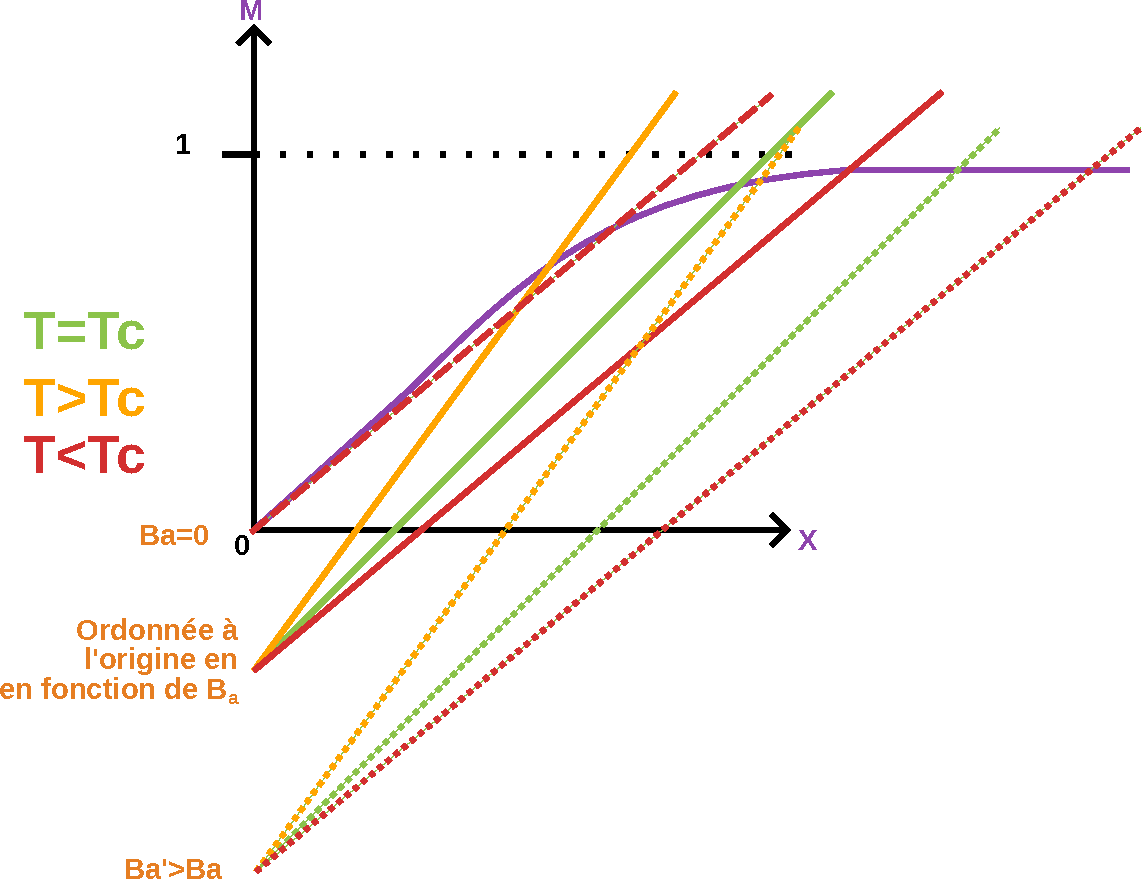
\includegraphics[scale=0.5]{courbes.pdf}

L'agitation thermique augmente et empêche les moments magnétiques de s'aligner sur $B_a$ Les probabilités d'occupation des états $\pm \mu_b$ sont de + en + semblables.

Il faut que $T<T_c$.

On peut tracer le diagramme de phase :

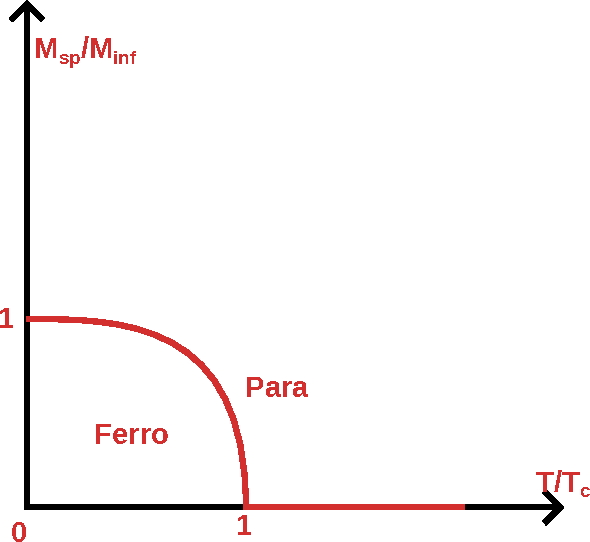
\includegraphics[scale=0.5]{msp.pdf}
\subsection{Retour l'énergie d'échange}
On cherche l'énergie d'intéraction entre 2 dipoles magnétiques : on ne souhaite qu'un ordre de grandeur.

L'énergie d'intéraction peut s'écrire $-\mu_2\cdot \vec{B_1}(A_2)$

Le champ crée par un dipole magnétique peut s'écrire dans le cadre de l'apprixmaiyion dipolaire : en injectant dans l'expression la formule, on obtient 

On fait les configurations pour $\vec{\mu_1}\perp \vec{r_{1/2}}$ et $\vec{\mu_2}\perp \vec{r_{12}} \Rightarrow \vec{mu_1}//\vec{\mu_2}$

L'énergie d'intéraction vaut $10^{-24}J\simeq 6e^{-6}eV$

Dans un réseau cubique, il y a 6 voisins donc on obtient 36eV.

On obtient une température de Curie mille fois trop petite.

D'où le besoin de la version quantique.
\end{document}